\section{Evaluations and Experimental Design}

\textit{Formative} \smallskip 

Early in the design process, sanity checks that we're building the right thing. 

\textit{Summative} \smallskip

Check if we improved upon our last iteration, does it work better than other solutions? \medskip

\textbf{Quantitative Evaluation Methods} \smallskip

Ensure certain level of quality, compare solutions objectively, attain a scientific statement. \medskip

\textbf{Primary Usability Metrics} \smallskip

\begin{center}
	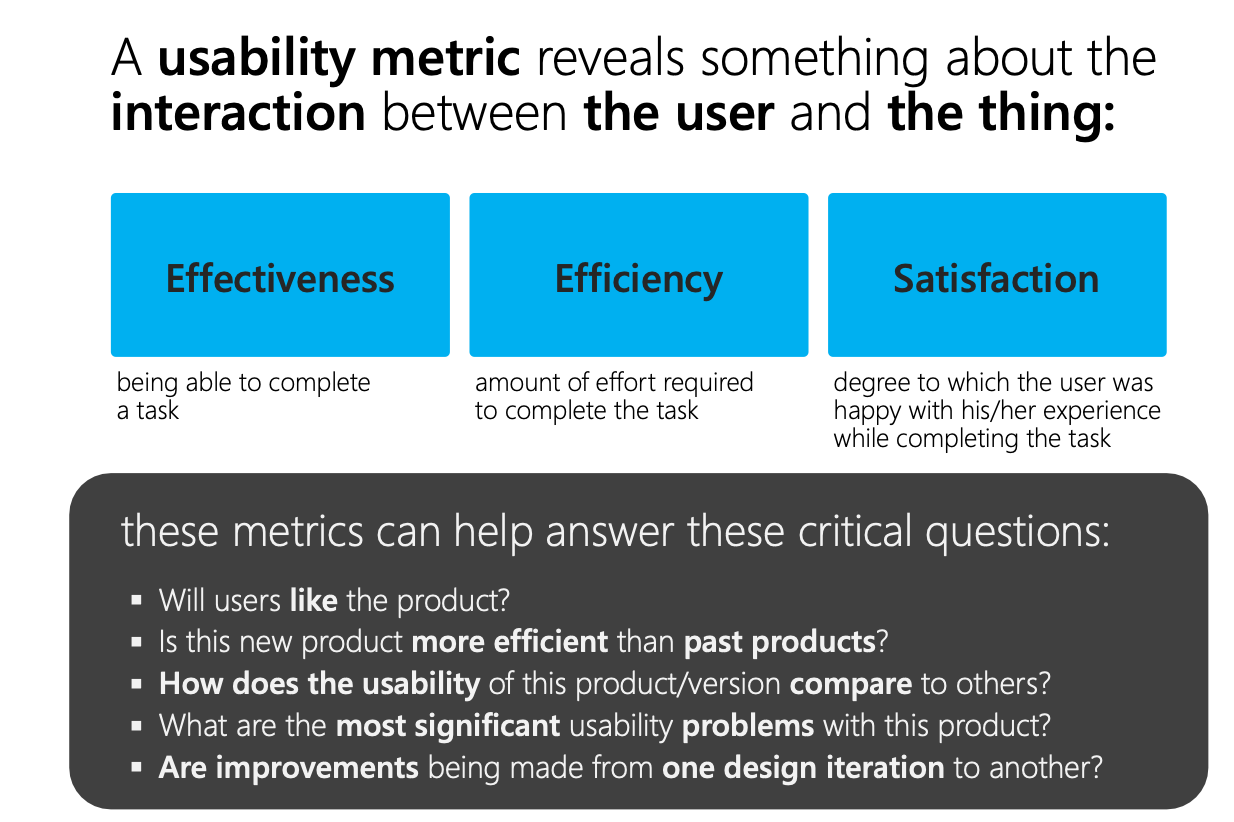
\includegraphics[width=\linewidth]{metrics.png}
\end{center}

\columnbreak

\textbf{Cause and Effect} \smallskip

We want to identify clear causal links. Cause precedes effect, they need to correlate and other explanations have to be ruled out. 
Isolate causality by conducting controlled experiments. Alter design with suspected cause absent (control) and present (experimental condition).
All other conditions should be identical. \medskip

\textbf{Quasiexperimental | Observational} \smallskip

We observe that independent variable and dependent variable are highly correlated, but did not control for anything (for instance participation in exercices and final exam grade). \medskip

\textbf{Experimental | Controlled} \smallskip

We randomly assign students to exercise and no exercise condition, then we control for other variables and results imply causality. \medskip


\textbf{characteristics of Emprical Methods}

\begin{itemize}
    \item Objectivity
    \item Reproducibility
    \item Validity (internally and externally)
    \item Relevance
\end{itemize}

For instance threat to external validity is over-use of specific participant groups (only psychology or cs students). \medskip

Threat to internal validity is any influence questioning causality. 


\textbf{The experiment}

Independent variables affect the dependent (measured) variables through experiment.

Variables can be catagorical, ordinal (ordered discrete), or cardinal/interval (continuous) data. \medskip

\textbf{Designing an empirical study}

\begin{enumerate}
    \item What is being compared? (which Independent variables)
    \item What are they being compared in? (dependent variables, metrics)
    \item What else is being varied? (extraneous variables to control/eliminate)
    \item Relevance
\end{enumerate}

Look at slide set 5 for various examples. \medskip

\textbf{More complex comparisons}

Different experimental designs possible: \textit{Within subjects:} Everyone-does everything. \textit{Between subjects:} Only one condition per group. \medskip

\textbf{Latin Square Counterbalancing}

\begin{center}
	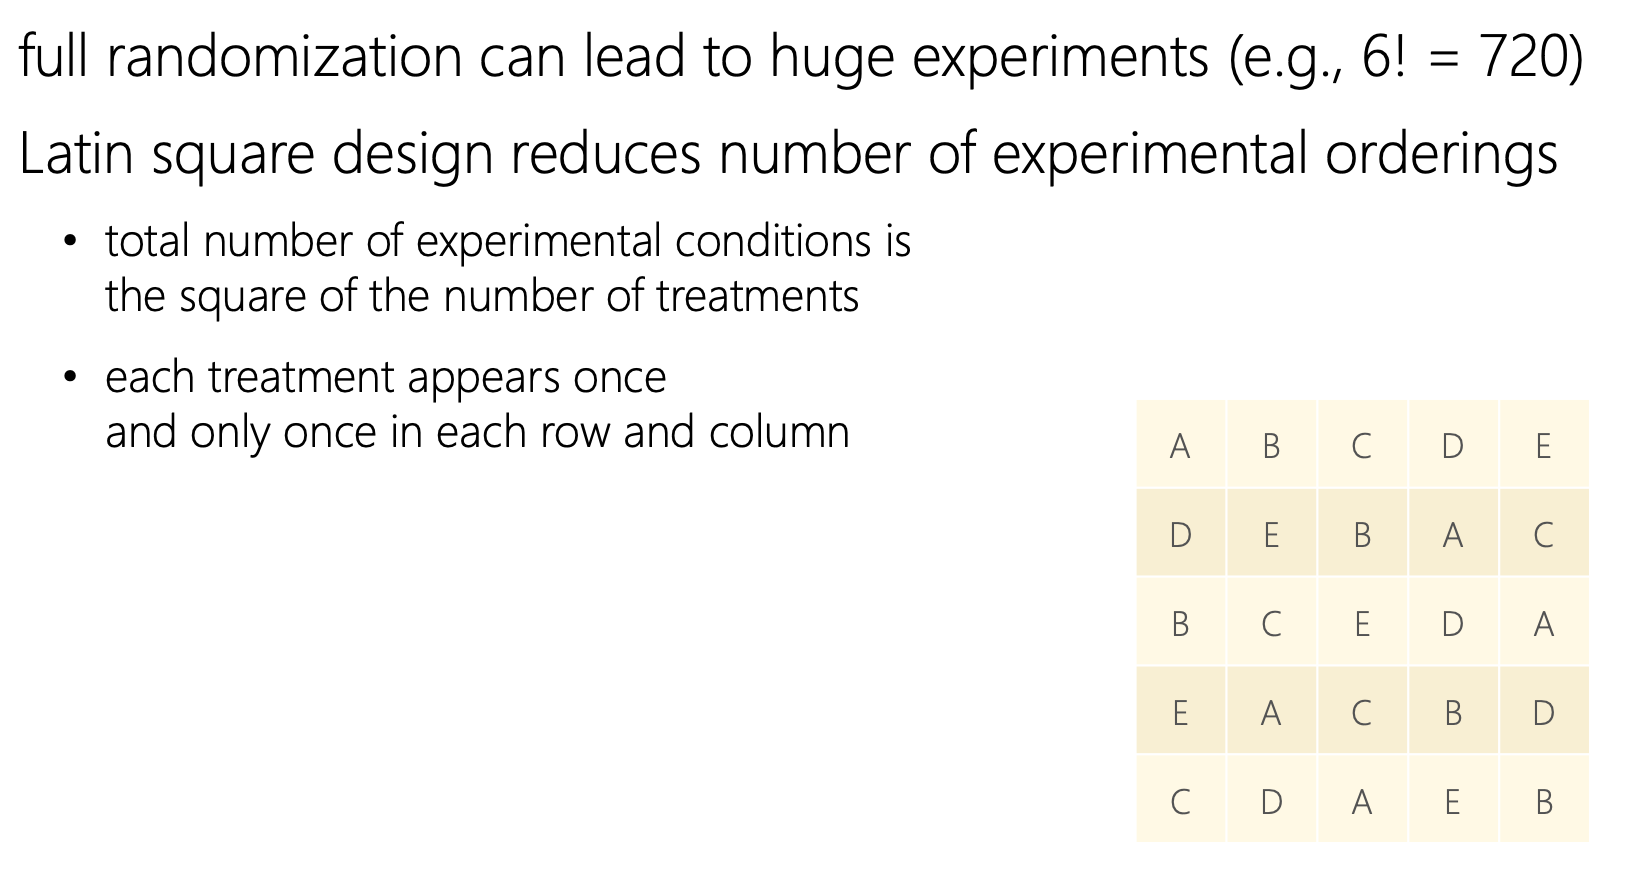
\includegraphics[width=\linewidth]{latin_square.png}
\end{center}


\textbf{Latin Square Example for 5}

\begin{center}
	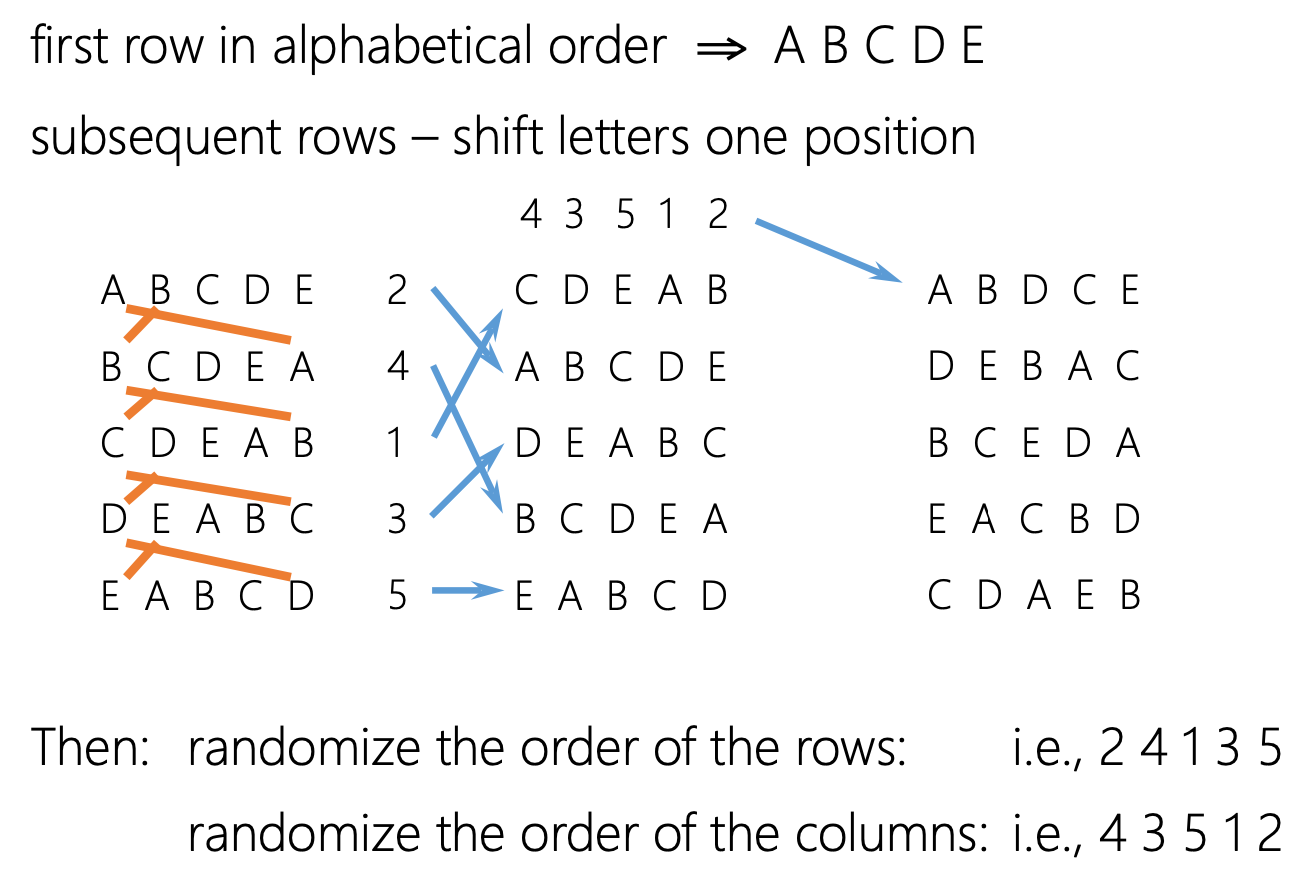
\includegraphics[width=\linewidth]{latin_example.png}
\end{center}

\columnbreak